\documentclass[12pt]{article}
\usepackage[T2A]{fontenc}
\usepackage[utf8]{inputenc}
\usepackage[russian]{babel}
\usepackage{secdot}

\textheight=24cm
\textwidth=16cm
\oddsidemargin=0pt
\topmargin=-1.5cm
\parindent=24pt
\parskip=0pt
\tolerance=2000
\flushbottom

\usepackage{amsmath}
\usepackage{amssymb}
\usepackage{amsthm}
\usepackage[]{algorithm2e}
\usepackage[shortlabels]{enumitem}
\theoremstyle{definition}
\usepackage{float}
\usepackage{graphicx}

\title{Сложность вычислений. \\
Вероятностная проверка на простоту без ошибок}
\date{}
\author{Константин Чернис, группа 694}

\newtheorem*{Def*}{Определение}
\newtheorem*{Th*}{Теорема}

\newtheorem{Def}{Определение}
\newtheorem{Th}{Теорема}
\newtheorem{St}{Утверждение}
\newtheorem{Cor}{Следствие}

\numberwithin{Def}{section}
\numberwithin{Th}{section}
\numberwithin{St}{section}
\numberwithin{Cor}{section}

\newenvironment{Proof}                    
        {\par\noindent{\bf Доказательство.}}
        {\hfill$\scriptstyle\blacksquare$}

\newcommand{\Set}[2]{
  \{\, #1 \mid #2 \, \}
}

\begin{document}
\begin{titlepage}
	\centering
	{\scshape\Large Сложность вычислений\par}
	\vspace{1.5cm}
	{\huge\bfseries Вероятностная проверка на простоту без ошибок\par}
	\vspace{2cm}
	{\Large Чернис Константин, группа 694\par}
	\newpage
\end{titlepage}
\tableofcontents
\newpage

В данном проекте доказываются избранные факты вероятностной
проверки чисел на простоту, а также проводятся некоторые 
эксперименты.

\section{Введение в сложностные классы}

Для начала опишем сложностные классы, затрагиваемые данной задачей:

\begin{Def}
	Вероятностной машиной Тьюринга называется детерминированная машина Тьюринга $M$ с
	двумя аргументами $x$ (аргумент вероятностной машины) и $r$ (случайные биты), где
	длина $r$ есть некоторая функция от длины $x$. Результатом работы $M$ на входе $x$
	будет вероятностое распределение, индуцированное данным $x$ и равномерным на всех
	значениях $r$. Временем работы $M$ на данном $x$ будем считать максимальное время работы
	$M(x,r)$ для всех $r$ указанной длины. Так же определяется и использованная память.
\end{Def}

\begin{Def}
	Классом \textbf{RP} называется класс языков $A$, для которых существует полиномиальный
	в худшем случае вероятностный алгоритм $V$, такой что:
	
	\begin{itemize}
		\item если $x\in A$, то $P_r[V(x,r)=1]\geqslant\dfrac 12$;
		\item если $x\notin A$, то $P_r[V(x,r)=1]=0$.
	\end{itemize}
\end{Def}

\begin{Def}
	Классом \textbf{coRP} называется класс языков $A$, для которых существует полиномиальный
	в худшем случае вероятностный алгоритм $V$, такой что:
	
	\begin{itemize}
		\item если $x\in A$, то $P_r[V(x,r)=1]=1$;
		\item если $x\notin A$, то $P_r[V(x,r)=1]\leqslant\dfrac 12$.
	\end{itemize}	
\end{Def}
	
\begin{Def}
	Классом \textbf{ZPP} называется класс языков $A$, для которых существует
	вероятностный алгоритм $A$, такой что
	$$
	x\in A\iff\forall r\; V(x,r)=1,
	$$
	а для каждого $x$ ожидаемое по $r$ время работы полиномиально.
\end{Def}

Обозначение \textbf{ZPP} расшифровывается как "zero-error probabistic
polynomial".

\begin{St}
	$\mathbf{ZPP=RP\cap coPR}$.
\end{St}

Таким образом, для вероятностной проверки чисел на простоту достаточно
предоставить алгоритмы проверки чисел на простоту из \textbf{RP} и \textbf{coRP},
после чего запускать их по очереди до тех пор, пока один из алгоритмов
не выдаст ответ, в котором он уверен. Вероятность отсутствия ответа будет
уменьшаться минимум в 4 раза после каждой итерации цикла проверки, так что
за полиномиальное число шагов вероятность станет экспоненциально малой и можно
будет применить детерминированный экспоненциальный алгоритм.

\section{Сертификаты}

\begin{St}
	$\mathbf{RP\subset NP}$
\end{St}

\begin{Proof}
	Действительно, любое значение $r$, при котором $V(x,r)=1$, будет доказательством
	того, что $x\in A$.
\end{Proof}

\begin{Cor}
	$\mathbf{coRP\subset coNP}$
\end{Cor}

Таким образом, в силу того, что язык простых чисел, как будет показано далее,
лежит в \textbf{ZPP}, для любого $n\in \mathbb{Z}$ существует либо сертификат простоты,
либо сертификат того, что $n$ составное, проверяемый за полиномиальное время.
Таким образом, единожды проверив число на простоту за вероятностно полиномиальное
время, в дальнейшем можно снова доказать корректность проверки уже за детерминированный 
полином.
Эти сертификаты будут указаны для каждого описанного ниже алгоритма соответственно.

\paragraph{} В следующей секции будет описан алгоритм из \textbf{coRP}, а в
секции 4~"--- из \textbf{RP}.

\section{Алгоритм Миллера-Рабина}

Большинство алгоритмов вероятностной проверки на простоту из \textbf{coRP}
опираются на какое-либо свойство простых чисел, то есть проверяют необходимое
условие. Наиболее популярным среди них является алгоритм Миллера-Рабина, который
гарантирует, что для нечётного составного минимум $75\%$ чисел от $1$ до $n-1$
позволяют определить его непростоту.

Говоря в терминах Определения 1.3,
$A$~"--- множество простых чисел, и для
$x\notin A$ $P_r[V(x,r)=1]\leqslant\dfrac 14$, где $r\in\overline{1,n-1}$.
Кроме того, как будет показано ниже, проверяемое условие действительно
является необходимым, то есть для $x\in A$ $P_r[V(x,r)=1]=1$, то есть
алгоритм Миллера-Рабина лежит в \textbf{coNP}.

\subsection{Описание алгоритма}
\newcommand{\Mod}[1]{\ \mathrm{mod}\ #1}

Заданное нечётное целое число $n>1$ можно представить в виде $n-1=2^ek$,
где $e\geqslant 1$ (т.к. $n$ нечётно) и $k$ нечётное. Применяя к
$x^{n-1}-1=x^{2^ek}-1$ формулу разности квадратов, получаем:
\begin{align*}
	x^{2^ek}-1&=\left(x^{2^{e-1}k}\right)^2-1 \\
	&=\left(x^{2^{e-1}k}-1\right)\left(x^{2^{e-1}k}+1\right) \\
	&=\left(x^{2^{e-2}k}-1\right)\left(x^{2^{e-2}k}+1\right)
	\left(x^{2^{e-1}k}+1\right) \\
	&\;\;\vdots \\
	&=\left(x^k-1\right)\left(x^k+1\right)\left(x^{2k}+1\right)
	\left(x^{4k}+1\right)\ldots\left(x^{2^{e-1}k}+1\right)
\end{align*}
Если $n$ простое и $a\in\overline{1,n-1}$, то
по малой теореме Ферма $a^{n-1}-1\equiv 0\Mod{n}$. Используя разложение,
полученное выше, имеем
$$
\left(x^k-1\right)\left(x^k+1\right)\left(x^{2k}+1\right)
	\left(x^{4k}+1\right)\ldots\left(x^{2^{e-1}k}+1\right)\equiv 0\Mod{n}
$$
Таким образом, для простого $n$ один из множителей должен делиться на $n$,
то есть необходимым условием, нарушение которого означает, что число составное,
является
$$
a^k\equiv 1\Mod{n}\text{ или } a^{2^ik}\equiv -1\Mod{n} \text{ для некоторого } 
i\in\overline{0,e-1}.
$$

\begin{Def}
Представим нечётное $n>1$ в виде $n-1=2^ek$, где $e$ нечётно и выберем
$a\in\overline{1,n-1}$. Тогда $a$ называется свидетелем для числа $n$, если
не выполнено необходимое условие, то есть
$$
a^k\not\equiv1\Mod{n}\text{ и } a^{2^ik}\not\equiv-1\Mod{n}\;\forall 
i\in\overline{0,e-1}.
$$
Если же необходимое условие выполнено, то есть
$$
a^k\equiv 1\Mod{n}\text{ или } a^{2^ik}\equiv -1\Mod{n} \text{ для некоторого } 
i\in\overline{0,e-1},
$$
то $a$ не является свидетелем для $n$.
\end{Def}

Отметим, что уже сейчас можно построить вероятностный алгоритм проверки на
простоту со сколь угодно малой вероятностью ошибки:
\\\\
\begin{algorithm*}[H]
 \KwData{проверяемое число $n$, количество итераций $t$}
 \KwResult{является ли число $n$ простым}
  \For{$i \in\overline{1,t}$}{
  выбрать случайное $a$ из $\overline{1,n-1}$\;
  \If{$a$ является свидетелем для $n$}{
   \Return "n составное"\;
   }
 }
 \Return "$n$ простое с вероятностью минимум $1-1/4^t$"\;
\end{algorithm*}
 
\subsection{Доказательство оценки на число свидетелей}

Для начала покажем, что оценка $75\%$ неулучшаема:
 
\begin{St}
	Доля свидетелей для $n=9$ составляет $3/4$.	
\end{St}

\begin{Proof}
	$n-1=8=2^3$, так что $e=3$ и $k=1$, и для проверки необходимого условия
	надо перебрать $(a,a^2,a^3)$. Из приведённой ниже таблицы видно, что
	свидетелями среди $\overline{1,8}$ являются $2, 3, 4, 5, 6, 7$, что
	составляет $6/8=3/4$, что и требовалось.
	
	\begin{center}
	\begin{tabular}{ c|c|c|c|c|c|c|c|c}
    $a\Mod 9$   & $1$ & $2$ & $3$ & $4$ & $5$ & $6$ & $7$ & $8$ \\ \hline
    $a^2\Mod 9$ & $1$ & $4$ & $0$ & $7$ & $7$ & $0$ & $4$ & $1$ \\
    $a^3\Mod 9$ & $1$ & $7$ & $0$ & $4$ & $4$ & $0$ & $7$ & $1$
  \end{tabular}
\end{center}
\end{Proof}

Существует также доказательство неулучшаемости оценки при $n\to\infty$,
оно приведено в \ref{Monier}.

\begin{Th}
 	Пусть $n>1$ нечётное составное.
 
 	Доля целых чисел среди $\overline{1,n-1}$, являющихся свидетелями числа $n$,
 	превышает $75\%$, за исключением $n=9$, для которого доля составляет $75\%$.
 	
 	Другими словами, доля целых чисел среди $\overline{1,n-1}$, не являющихся
 	свидетелями числа $n$, меньше $25\%$, за исключением $n=9$, для которого доля 
 	составляет $25\%$.
\end{Th}

Докажем более слабое утверждение:

\begin{Th}
	Если $n>1$ нечётное и составное, то доля свидетелей числа $n$ превышает
	$50\%$. Другими словами, больше $50\%$ из $a\in\overline{1,n-1}$
	удовлетворяют $a^k\not\equiv 1\Mod{n}$ и
	$a^{2^ik}\not\equiv-1\Mod{n}\;\forall i\in\overline{0,e-1}$.
\end{Th}

\begin{Proof}
	Докажем, что доля не свидетелей для $n$ меньше $50\%$, показав, что они
	образуют собственную подгруппу группы обратимых чисел$\Mod{}n$. В силу того,
	что порядок собственной подгруппы составляет максимум половину от порядка
	группы, множество свидетелей числа $n$ содержит минимум половину обратимых
	чисел$\Mod{n}$ и все необратимые числа$\Mod{n}$ среди $\overline{1,n-1}$
	(множество необратимых непусто в силу того, что $n$ составное).
	Таким образом, доля свидетелей для числа $n$ первышает $50\%$.
	
	\textbf{Случай 1:} $n$ является степенью простого числа,
	то есть $n=p^\alpha$, где $p$ — нечётное простое и $\alpha\geqslant 2$.
	
	\begin{St}
		Если $n=p^\alpha$ для простого $p$ и $\alpha\geqslant 1$, то
		не свидетели для $n$ являются корнями уравнения
		$a^{p-1}\equiv 1\Mod{p^\alpha}$, которые образуют группу по
		умножению$\Mod{n}$.
	\end{St}
	
	\begin{Proof}
		Обоснование приведено в \ref{Conrad}.
	\end{Proof}
	\\\\
	Согласно Утверждению 2.2 свидетели непростоты образуют группу по умножению
	$\Mod{n}$. Порядок числа $a$, являющегося решением уравнения
	$a^{p-1}\equiv1\Mod{n}$, делит $p-1$, так что он не делится на $p$. В то же
	время существуют обратимые$\Mod{n}$ числа, порядок которых делится на $p$:
	примером такого числа является $1+p$, чей порядок$\Mod{p^\alpha}$ составляет
	$p^{\alpha-1}$ (этот факт можно показать индукцией по $r$: база~"---
	$1+kp\equiv 1\Mod{p}$, переход~"--- $(1+kp^r)^p\equiv 1\Mod{p^{r+1}}$).
	Таким образом, не свидетели$\Mod{n}$ образуют собственную подгруппу в группе
	обратимых чисел$\Mod{n}$, что заканчивает доказательство этого случая.
	\\\\
	\textbf{Случай 2:} $n$ не является степенью простого. Пусть
	$i_0\in\overline{0,e-1}$~"--- максимальное число, такое что
	$\exists\,a_0\in\mathbb{Z}$ такой что $a^{2^{i_0}}\equiv-1\Mod{n}$.
	(В силу того, что $(-1)^{2^0}=-1$, требуемый $i_0$ существует, причём
	$a_0$ взаимно прост с $n$).
		
	Множество
	$$
	G_n=\Set{a\in\overline{1,n-1}}{a^{2^{i_0}k}\equiv\pm1\Mod{n}}
	$$ 
	является группой по умножению$\Mod{n}$ и содержит все $a$, удовлетворяющие
	одному из двух условий:
	\begin{enumerate}[(1)]
		\item $a^k\equiv 1\Mod{n}$,
		\item $a^{2^ik}\equiv 1\Mod{n}$ для одного из $i\in\overline{0,e-1}$.
	\end{enumerate}
	
	Если $a^k\equiv 1\Mod{n}$, то $a^{2^{i_0}k}\equiv 1\Mod{n}$. Если же
	$a^{2^ik}\equiv 1\Mod{n}$ для некоторого $i\in\overline{0,e-1}$, то
	$\left(2^k\right)^{2^i}\equiv-1\Mod{n}$, причём $i\leqslant i_0$ в силу
	максимальности $i_0$. Таким образом, $a^{2^{i_0}}\equiv -1\Mod{n}$, если
	$i=i_0$, и $a^{2^{i_0}}=1\Mod{n}$, если $i<i_0$. Отсюда все
	$a\in\overline{1,n-1}$, удовлетворяющие (1) или (2), лежат в $G_n$.
	
	Покажем, что $G_n$ является собственной подгруппой обратимых чисел$\Mod{n}$,
	для чего найдём обратимое число, не лежащее в $G_n$. Пусть $p$~"--- простой
	делитель $n$, тогда представим $n$ в виде $n=p^\alpha n'$, где
	$\alpha\geqslant 1$ и $p\nmid n'$. $p^\alpha$ и $n'$ нечётные и не равны $1$
	(в силу того, что $n$ не является степенью простого) $\implies$
	$p^\alpha,n'\geqslant 3$.
	
	Согласно китайской теореме об остатках, $\exists\,a\in\overline{1,n-1}$,
	удовлетворяющий следующим двум уравнениям:
	$$
	a\equiv a_0\Mod{p^\alpha}, \quad a\equiv 1\Mod{n'}. 
	$$
	Выше показали, что $(a_0,n)=1\implies (a,n)=1$ (т.к. $(a,n')=1$), то есть
	$a$ является обратимым$\Mod{n}$. Тогда для доказательства того, что подгруппа
	$G_n$ не является собственной, остаётся показать, что $a\notin G_n$.
	
	$$
	a^{2^{i_0}k}\equiv a^{2^{i_0}k}_0 \equiv (-1)^k\equiv -1\Mod{p^\alpha}
	\implies a^{2^{i_0}k}\not\equiv 1\Mod{n}
	$$
	в силу того, что $-1\not\equiv 1\Mod{p^\alpha}$ (т.к. $p^\alpha\geqslant 3$).
	Кроме того,
	$$
	a^{2^{i_0}k}\equiv 1\Mod{n'}\implies a^{2^{i_0}k}\not\equiv -1\Mod{n}
	$$
	в силу того, что $-1\not\equiv 1\Mod{n'}$ (т.к. $n'\geqslant 3$). Таким
	образом, $a\notin G_n$, что завершает доказательство данного случая, а с ним
	и всей теоремы.
\end{Proof}
\\\\
Теорема 2.1 доказазывается аналогичным образом, оценка $1/4$ на число
не свидетелей достигается за счёт двукратного применения приёма с собственной
подгруппой. Полное доказательство описано в \ref{Conrad}.

\subsection{Сертификат}

Из алгоритма видно, что сертификатом является определённый выше свидетель~"---
число $a$, для которого не выполнено необходимое условие простоты. Сложность
проверки сертификата составляет $O(\log^3 n)$, если умножение производится
за $O(\log^2n)$, то есть проверка сертификата полиномиальна.

\paragraph{} На самом деле, для большинства составных чисел доля свидетелей
гораздо выше $75\%$. Для демонстрации этого факта построим гистограмму долей
свидетелей для всех составных чисел до $10^4$:

\begin{figure}[H]
 	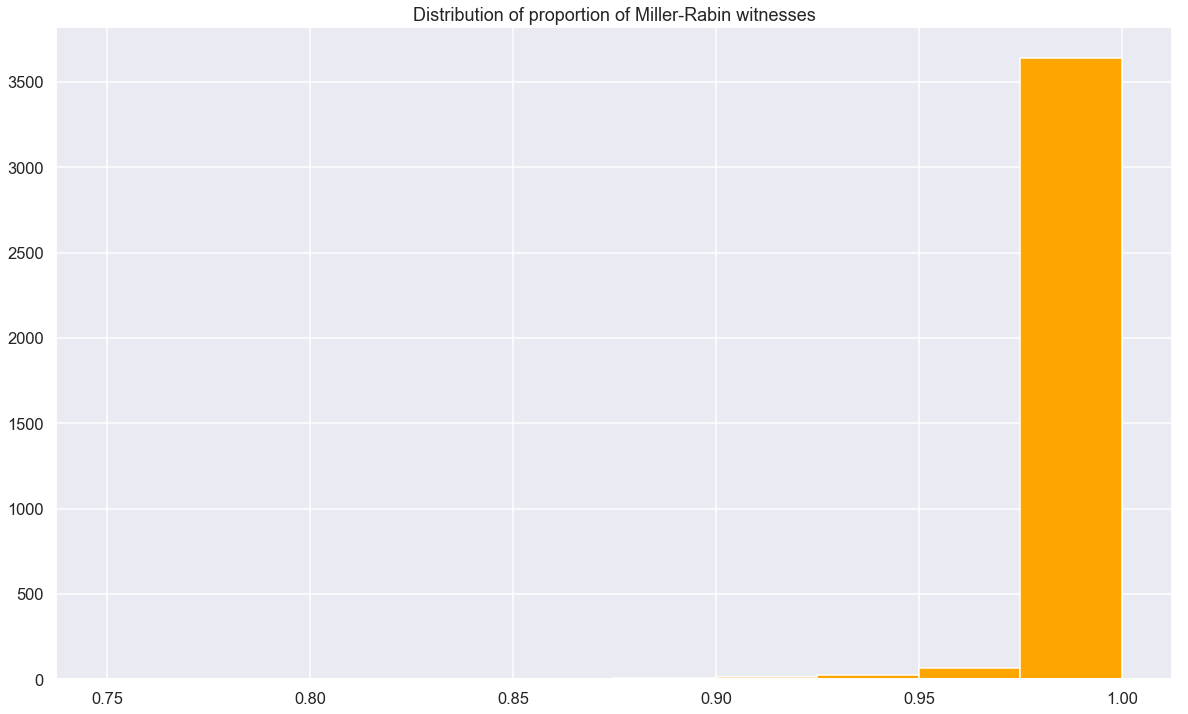
\includegraphics[width=\linewidth]{miller-rabin.png}
\end{figure}

\paragraph{}В следующей секции будет описан алгоритм из \textbf{RP}. В силу
нетривиальности оного будет дано неформальное интуитивное описание. Полный
алгоритм и доказательство корректности доступно в \ref{Adleman}.

\section{Алгоритм Эдельмана-Хуана}

Для начала проиллюстрируем метод проверки на простоту, используемый в алгоритме
Эдельмана-Хуана.

\subsection{Пример}

Рассмотрим следующее доказательство простоты числа 11:
\begin{enumerate}[(1)]
	\item $(4-1,11)=1$
	\item $4^5=1024\equiv1\Mod11$
	\item 5~"--- простое число
\end{enumerate}
Пусть 11 не является простым. Тогда существует простое $p\leqslant\sqrt{11}<4$,
делящее 11. Из (1) получаем, что
$4\Mod p\not\equiv1$ в $Z/pZ^*\implies ord(4\Mod p)\neq 1$. Из (2) следует,
что $ord(4\Mod p)\mid 5$. Наконец, из (3) получаем, что $ord(4\Mod p)=5$,
что невозможно, так как $p<4$.

Заметим, что без (3) рассуждение выше дало бы сведение доказательства простоты
числа 11 к простоте числа 5. Идея сведения доказательства простоты одного числа
к простоте другого является ключевой в описываемом алгоритме.

\paragraph{}Построим алгоритм на технике из примера:

\paragraph{Алгоритм:} Для достаточно больших $p$ за
вероятностно полиномальное время можно свести
доказательство простоты $p$ к простоте $\dfrac{p-1}2$. Для этого надо лишь
перебирать случайные $a\in Z_{>0}$, пока не будет выполнено
\begin{enumerate}[(1)]
	\item $(a-1,p)=1$
	\item $a^{\frac{p-1}2}\equiv1\Mod p$
\end{enumerate}

Для $p>2$ существует $\dfrac{p-3}2$ чисел $a<p$, удовлетворяющих этим
требованиям, так что алгоритм будет работать за вероятностно полиномиальное
время.

Возвращаясь к проверке на простоту числа 11, можно было свести простоту числа 5
к простоте числа 2, которую можно проверить явно. В то же время данный алгоритм
не применим в общем случае, ибо сведение простоты числа 13 к простоте числа 6
бесполезно.

\paragraph{} В следующем подпункте будет описан рабочий алгоритм, обеспечивающий
сведение.

\subsection{Алгоритм Гольдвассер-Килиана}

Алгоритм Гольдвассер-Килиана обходит описанную выше проблему за счёт
использования групп, отличных от $Z/pZ^*$. Для этого введем эллиптические кривые:

\begin{Def}
Эллиптической кривой называется кривая, задаваемая уравнением вида
$$
y^2=x^3+Ax+b,
$$
для которой выполнено $\Delta=4A^3+27B^3\neq 0$.
\end{Def}


\paragraph{Алгоритм:} Случайным образом ищем $a,b\in Z/pZ$, удовлетворяющие
следующим условиям:
\begin{enumerate}[(1)]
	\item $f(x)=x^3-ax+b$ не имеет кратных корней
	\item число рациональных точек на эллиптической кривой $y^2=f(x)$ равно
	$2*m$ для некоторого $m\in Z$
\end{enumerate}
Далее ищем пару $s,t\in Z/pZ$, таку что
\begin{enumerate}[(1)]
	\item точка $v=\langle s,t\rangle$ лежит на кривой
	\item $m*v=1$ в группе, ассоциированной с кривой
\end{enumerate}

Можно показать, что что если найти $v$, удовлетворяющую условию, то
доказательство простоты $p$ сводится к доказательству простоты $m$ (то есть
получено утверждение $m\text{ простое}\implies p\text{ простое}$). Кроме того,
из гипотезы Римана для конечных полей $m\approx\dfrac p2$.

С другой стороны, для того, чтобы описанный выше алгоритм был вероятностно
полиномиальным, требуется, чтобы на случайно сгенерированной эллиптической кривой
с высокой вероятностью было дважды простое число рациональных точек. Гипотеза
Римана гарантирует, что число точек находится в интервале
$$
[p+1-2\sqrt{p},p+1+2\sqrt{p}]
$$
В силу того, что этот интервал слишком мал, вероятностная полиномиальность
описанного выше алгоритма до сих пор не доказана. Эта проблема решена в алгоритме
Эдельмана-Хуана, описанном ниже.

\subsection{Алгоритм Эдельмана-Хуана}

Введём понятие гиперэллиптических кривых:

\begin{Def}
	Гиперэллиптической кривой рода $g>1$ называется алгебраическая кривая,
	задаваемая уравнением вида
	$$
	y^2+h(x)y=f(x),
	$$
	где $f(x)$~"--- многочлен степени $n=2g+1>4$ или с $n=2g+2>4$ различными
	корнями и $h(x)$~"--- многочлен степени $<g+2$.
\end{Def}

Для расширения множества чисел, для которых существует сведение, описанное
в предыдущем пукте, в алгоритме Эдельмана-Хуана используется обобщённый
алгоритм Гольдвассер-Килиана. Кроме того, вводится сведение нового типа:
в нём эллиптические кривые заменяются на матрицы Якоби гиперэллиптических
кривых второго рода. Тогда сведение нового типа вычисляется за вероятностно
полиномиальное время следующим образом:

\paragraph{Алгоритм:}
\begin{enumerate}[1)]
	\item Случайным образом ищем многочлен $f\in Z/pZ[x]$ степени 6,
который не имеет кратных корней.
	\item Считаем число $n$ рациональных точек на матрице Якоби кривой,
	задаваемой уравнением $y^2=f(x)$
	\item Находим такие $s,t\in Z/pZ, t\neq0$, что точка $\langle s,t \rangle$
	лежит на кривой и ${v=\langle s,t\rangle-\langle s,-t \rangle}$ (или, точнее,
	${v=\phi(\langle s,t\rangle)-\phi(\langle s,-t \rangle)}$, где $\phi$~"---
	вложение кривой в группу матриц Якоби) удовлетворяет равенству $n*v=1$ в 
	группе, ассоциированной с матрицами Якоби.
\end{enumerate}

Получаем сведение доказательства простоты $p$ к доказательству простоты $n$,
которое, как и раньше, работает только если $n$~"--- простое. В силу того,
что $n$ простое с высокой вероятностью, новый алгоритм является вероятностно
полиномиальным.

С другой стороны, в силу гипотезы Римана для конечных полей $n\approx p^2$.
Таким образом, алгоритм Эдельмана-Хуана обходит числа, для которых не выходит
получить сведение с помощью обобщённого алгоритма Гольдвассер-Килиана, производя
несколько итераций нового сведения. В силу почти случайного выбора $n$ данный
способ позволяет избежать чисел из плохого множества.

Для завершения построения алгоритма остаётся научиться быстро считать число
рациональных точек на эллиптических кривых, алгоритм Шуфа \ref{Schoof}
справляется с этой задачей за полиномиальное время. Получаем

\begin{Th}
	Существует $c\in Z_{\geqslant 0}$ и полиномиально вычислимая всюду
	всюду определённая функция $F:Z^2_{\geqslant 0}\to \{0,1\}$, такая что
	\begin{enumerate}
		\item $\forall n\in Z_{\geqslant 0}$, где $n$ составное, и
		$\forall r\in Z_{\geqslant 0}$
		$$
		F(n,r)=0
		$$
		\item $\forall p\in Z_{\geqslant 0}$, где $p$ простое,
		$$
		\dfrac{\#\{r:|r|\leqslant|p|^e\text{ и }F(n,r)=1\}}
		{\#\{r:|r|\leqslant|p|^e\}}\geqslant\dfrac 12,
		$$
	\end{enumerate}
	то есть проверка на простоту лежит в \textbf{RP}. Учитывая, что в секции 3
	было показано, что эта задача лежит в \textbf{coRP}, получаем, что она лежит
	в $\mathbf{ZPP=RP\cap coPR}$.
\end{Th}

\subsection{Сертификат}

В данном случае сертификатом является последовательность чисел, к которым
производится сведение доказательства простоты в процессе работы алгоритма,
а для его проверки требуется лишь проверить корректность сведений и 
проверить полученное небольшое число на простоту делением на все числа
в интервале $[2, \sqrt{n}]$, что делается за полином.

Наконец, рассмотрим наиболее эффективный на данный момент \textbf{RP} алгоритм
проверки на простоту, алгоритм Аткина-Морейна.

\section{Алгоритм ECPP}

\subsection{Описание}

Алгоритм ECPP построен на идее сведений, аналогичной алгоритму
Гольдвассер-Килиана, но для ускорения отказывается от использования 
неэффективного алгоритма Шуфа для подсчёта числа рациональных точек на
эллиптической кривой. Вместо этого с помощью комплексного умножения
случайно генерируется кривая, число рациональных точек на которой легко 
подсчитать.

Сведения в алгоритме ECPP основаны на следующей теореме:

\begin{Th}
Пусть $N\in\mathbb{N}_+$, и эллиптическая кривая $E$ задаётся уравнением
$$
y^2=x^3+ax+b\Mod N
$$
Рассматрим $E$ над $\mathbb{Z}/N\mathbb{Z}$, используя обычный закон сложения
и считая $0$ нейтральным элементом на $E$.

Пусть $m$ целое. Если существует простое число $q$, делящее $m$ большее, чем
${\left(\sqrt[4]{N}+1\right)^2}$ и на $E$ существует точка $P$,
для которой выполнено
\begin{enumerate}[(1)]
	\item $mP=0$
	\item (m/q)P определено и не равно $0$,
\end{enumerate}
то N простое.
\end{Th}

\subsection{Сертификат}

В силу того, что ECPP, также как и Гольдвассер-Килиан, производит цепочку
сведений, он также создаёт сертификат, хоть и не является вероятностно
полиномиальным

\subsection{Время работы}

Эвристическая (но не доказанная) асимптотика ECPP равна $O(\log^4 n)$.
Продемонстрируем это, построив зависимость $time$ от $\log\log n$:

\begin{figure}[H]
 	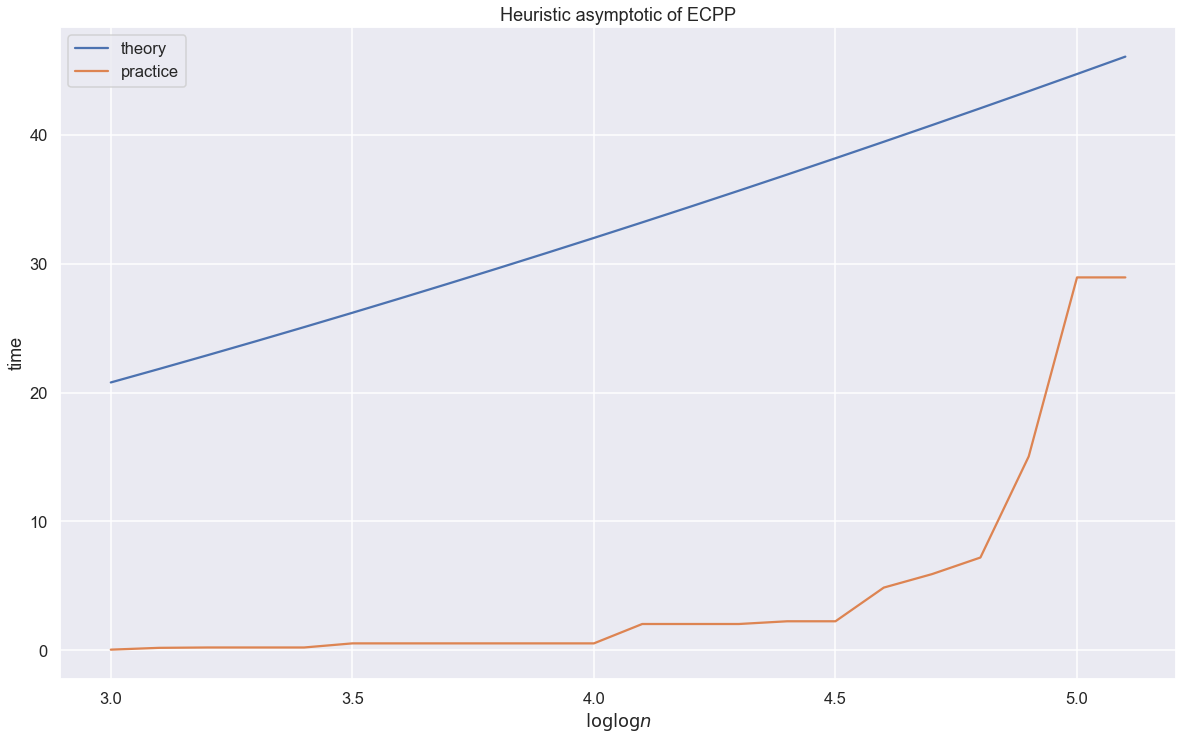
\includegraphics[width=\linewidth]{ecpp.png}
\end{figure}

\section{Практика}

На практике для проверки на простоту достаточно по очереди запускать
алгоритм Миллера-Рабина и ECPP, пока один из них не выдаст ответ без ошибки.
Чтобы получить вероятностно полиномиальный алгоритм, можно также параллельно
запустить алгоритм Эдельмана-Хуана.

\section{Список литературы}

\begin{enumerate}[{[}1{]}]
	\item Д.В. Мусатов. “Сложность вычислений.”
	\item \label{Conrad} Conrad, Keith. (2017). “The Miller – Rabin Test.”
	\item \label{Monier} Monier, Louis. (1980). "Evaluation and comparison of two efficient
	probabilistic primality testing algorithms."
	Theoretical Computer Science. 12. 97–108.
	\item \label{Adleman} M. Adleman, Leonard \& A. Huang, Ming-Deh. (1992).
	"Primality Testing and Abelian Varieties Over Finite Fields."
	10.1007/BFb0090185.
	\item \label{Schoof} Schoof, René. "Counting points on elliptic curves over 
	finite fields." Journal de théorie des nombres de Bordeaux 7.1 (1995): 
	219-254. <http://eudml.org/doc/247664>.
	\item Atkin, A. O. L., \& Morain, F. (1993). "Elliptic curves and primality 
	proving." Mathematics of Computation, 61(203), 29–29.
	doi:10.1090/s0025-5718-1993-1199989-x
\end{enumerate}

\end{document}